\chapter{Соревнования  «Сумо»}
{\bfseries Анонс:}\\\\
Соревнования простейших сумоистов. Анализ проблем устойчивости конструкций. Сила трения, центр тяжести, устойчивость.\\\\
{\bfseries Цели:}
\begin{itemize}
	\item{}{\bfseries Обучающие:} Закрепить понятия передаточного соотношения. Улучшить навыки конструирования. Добиться формулировки и понимания основных законов равновесия и устойчивости конструкции.
	\item{}{\bfseries Развивающая:} Сформировать умение прослеживать причинно-следственные связи.\\
\end{itemize}	
{\bfseries Ход занятия:}\\\\
\begin{tabular}{lll}
	\hyperlink{lesson8x1}{1. Организационный момент} & Презентация & (5 мин)\\
	\hyperlink{lesson8x2}{2. Соревнования  «Сумо»} & Игра & (60 мин) \\
	\hyperlink{lesson8x3}{3. Проблемы устойчивости} & Рефлексия & (10 мин) \\
	\hyperlink{lesson8x4}{4. Центр тяжести} & Презентация & 40 мин)\\
\end{tabular}\\\\

{\hypertarget{lesson8x1}{\blackBlueText{I. Организационный момент}}}\\\\
\\\\

{\hypertarget{lesson8x2}{\blackBlueText{II. Соревнования «Сумо»}}}\\\\

Учащиеся делятся на команды по 2--3 человека. Каждой команде предлагается придумать свое название, все команды вносятся в турнирную таблицу (рисуется на доске или проецируется на экран с компьютера), по принципу каждый с каждым.

Каждая команда получает задание~--- за 20 минут собрать на основе стандартной тележки и придуманных понижающих передач робота, который перетолкает соперника.\\\\

{\bfseries Регламент состязаний:}
\begin{enumerate}
	\item Робот должен быть собран на основе стандартной трехколесной тележки, но допустимы надстройки на нее.
	\item Программа робота пишется на блоке, одинакова для всех участников и представляет собой: Forward\(\to\)Empty\(\to\)Forward\(\to\)Empty\(\to\)Loop.
	\item В стартовой позиции роботы стоят напротив друг друга на расстоянии 10 см.
	\item По команде «Старт» участники запускаю программу на своих роботов. После этого вмешиваться в работу роботов запрещено!
	\item \label{sumoVinner}Победа присуждается роботу, который протолкал своего соперника более 10 секунд подряд.
	\item Если роботы находятся в контакте и не двигаются более 15 секунд, присуждается ничья.
	\item За победу команда получает 2 очка, за ничью 1 очко, за проигрыш~--- 0 очков.
	\item После проведения отборочных матчей В полуфинал проходят 2 команды с наибольшим количеством очков.
\end{enumerate}

{\slshape При большом количестве команд разумно провести 2 полуфинала, финал и матч за третье место.
	
	Матчи можно проводить на специальном поле (см. Приложение), тогда пункт \ref{sumoVinner} может выглядеть таким образом:  Победа присуждается роботу, который вытолкал своего противника за пределы круга.}\\\\

{\hypertarget{lesson8x3}{\blackBlueText{III. Проблемы устойчивости}}}\\\\	

После соревнований проводится анализ технических решений, приводивших команды к успеху или проигрышу, причем ценен любой опыт.
\begin{enumerate}
	\item Использовали ли вы понижающую передачу?
	\item Каково было передаточное соотношение у вас? У ваших соперников? 
	\item Буксовал ли ваш робот? Как этого можно было избежать?
	\item Покажите ведущие колеса вашего робота? Где сосредоточена основная масса вашего робота?
	\item Легко ли переворачивается ваш робот? Как можно сделать робота устойчивее?
\end{enumerate}

{\hypertarget{lesson8x4}{\blackBlueText{IV.  Центр тяжести}}}\\\\

Можно заметить, что некоторые роботы буксовали, т.е.  мощность двигателя расходовалась впустую. Что бы такого не происходило, запомним важное правило: {\bfseries основной вес робота должен приходится на ведущие колеса}. Оказывается, что чем больше давление, оказываемое колесом, тем больше трение между колесом и поверхностью, а значит и сцепление с поверхностью.

Возможно, вы заметили, что некоторые роботы легко переворачивались. Попробуем сформулировать законы равновесия и выяснить, как собрать устойчивого робота. Поэкспериметируем с равновесием. Встанем прямо, ноги вместе и попробуем немного отклониться. Ой, падаем! Как бы встать поустойчивее? Достаточно расставить ноги чуть пошире, на ширину плеч.

Получается, чем шире основание, тем устойчивее предмет? На первый взгляд похоже на правду, пирамиду явно сложнее уронить, когда она стоит основанием, а не вершиной на земле.
\begin{figure}[h!]
	\begin{center}
		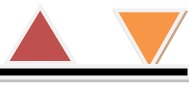
\includegraphics[width=0.35\linewidth]{chapters/chapter8/images/1}
		\caption{}
		\label{ris:image8x1}
	\end{center}
\end{figure}

Но маленький цилиндр явно устойчивее большого, хотя площади опоры у них и одинаковы. Получается дело не в опоре или не только в ней?
\begin{figure}[h!]
	\begin{center}
		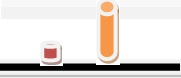
\includegraphics[width=0.35\linewidth]{chapters/chapter8/images/2}
		\caption{}
		\label{ris:image8x2}
	\end{center}
\end{figure}

Проведем такой опыт: положим пустой коробок на стол, а в него положим  тяжелую гайку. Сдвинем ее как можно ближе к одному краю. Теперь этот край будет удерживаться на столе, даже если почти весь коробок висит в воздухе.
\begin{figure}[h!]
	\begin{center}
		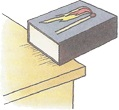
\includegraphics[width=0.5\linewidth]{chapters/chapter8/images/3}
		\caption{}
		\label{ris:image8x3}
	\end{center}
\end{figure}

Т.е. если основная масса тела находится над опорой тело не упадет? Хорошая догадка, но как понять где сосредоточена «основная масса» однородного цилиндра? 

Оказывается, чтобы строго сформулировать закон равновесия необходимо ввести понятие центра тяжести. {\bfseries Центром тяжести} механической системы называется точка, относительно которой суммарный момент силы, действующих на систему, равен нулю. 

{\slshape Тут необходимо лирическое отступление. Формально, понятие момента силы могло звучать у детей на уроке физики еще в 7 классе, при изучении темы «Рычаги». Однако, опыт показывает, что разъяснение определение в таком виде, как оно дано выше,  восьми – и девятиклассникам требует глубокого отступления и напоминания понятий сила, момент силы, правила моментов и решения задач на статику. А главное, в курсе робототехнике это, в отличие от кинематики вращательного движения, подробно расписанной выше, не сильно пригодится. Достаточно будет понимания того, что не стоит задирать тяжелые блоки робота наверх конструкции. Поэтому дальнейший текст написан в расчете на то, что перед младшими можно помахать руками и сказать что-то туманное о «точке, около которой сосредоточена основная масса тела». Категорически неверно, но в тандеме с предлагаемыми опытами формирует понимание этого понятия «на пальцах».}

Центр тяжести шара находится в центре, цилиндра – на половине высоты, кольца – в центре кольца, т.е. центр тяжести не обязан находится внутри самого тела. Центр тяжести человека обычно расположен в районе живота.
\begin{figure}[h!]
	\begin{center}
		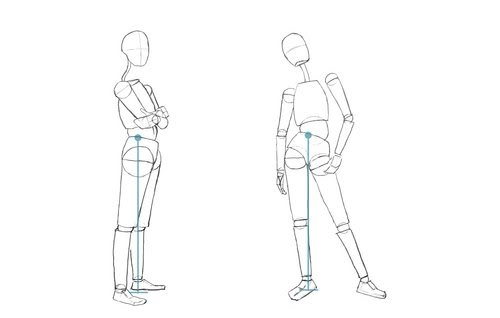
\includegraphics[width=1\linewidth]{chapters/chapter8/images/4}
		\caption{Центр масс человека}
		\label{ris:image8x4}
	\end{center}
\end{figure}	 

А искомый закон равновесия можно сформулировать так: {\bfseries перпендикуляр, опущенный из центра тяжести должен попадать в площадь опоры}. 
\begin{figure}[h!]
	\begin{center}
		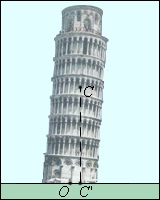
\includegraphics[width=0.45\linewidth]{chapters/chapter8/images/5}
		\caption{}
		\label{ris:image8x5}
	\end{center}
\end{figure}

Применим этот закон, к нашим опытам. Человек будет стоять, не падая, до тех пор пока перпендикуляр опущенный из его центра масс не выйдет за площадь опоры. Понятно, что расставляя ноги шире мы увеличиваем площадь опоры и нас сложнее уронить.
\begin{figure}[h!]
	\begin{center}
		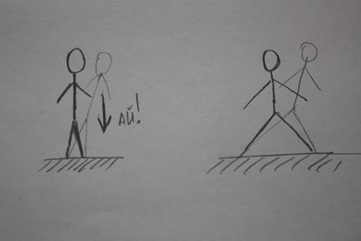
\includegraphics[width=0.75\linewidth]{chapters/chapter8/images/6}
		\caption{}
		\label{ris:image8x6}
	\end{center}
\end{figure}

У высокого цилиндра и центр тяжести оказывается выше. Таким образом его надо отклонить на меньший угол, что бы перпендикуляр, опущенный из центра масс вышел за площадь опоры. Это мы и подразумеваем под словом «устойчивее».
\begin{figure}[h!]
	\begin{center}
		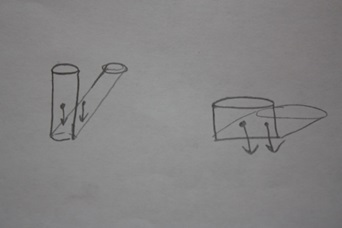
\includegraphics[width=0.75\linewidth]{chapters/chapter8/images/7}
		\caption{}
		\label{ris:image8x7}
	\end{center}
\end{figure}

На самом деле, есть еще один случай, когда тело будет находится в состоянии устойчивого равновесия. Проведем следующий опыт. Попробуем поставить карандаш на острие. Не получается? Не удивительно, площадь опоры-то малюсенькая и при любом самом незначительном наклоне, перпендикуляр, опущенный из центра масс, выходит за площадь опоры.

Но есть один старинный фокус, как заставить карандаш стоять на острие. В него надо воткнуть перочинный нож, как показано на рисунке.
\begin{figure}[h!]
	\begin{center}
		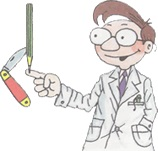
\includegraphics[width=0.2\linewidth]{chapters/chapter8/images/8}
		\caption{}
		\label{ris:image8x8}
	\end{center}
\end{figure}

Минутку, а где же находится центр тяжести подобной системы? Очевидно, что нож тяжелее карандаша, так что центр тяжести находится где-то под пальцем, ПОД опорой. И мы можем сформулировать дополнение к нашему закону равновесия: {\bfseries равновесие будет устойчиво, если центр тяжести находится ниже точки опоры}.

Так что на канатных дорогах в горах можно кататься совершенно спокойно, ведь кабинка висит под тросом и главная тяжесть находится ниже точки опоры. На основе этого же закона в одном из технических музеев Финляндии есть аттракцион~--- велосипед, на котором каждый может проехаться по тросу  высоко над землей.
\begin{figure}[h!]
	\begin{center}
		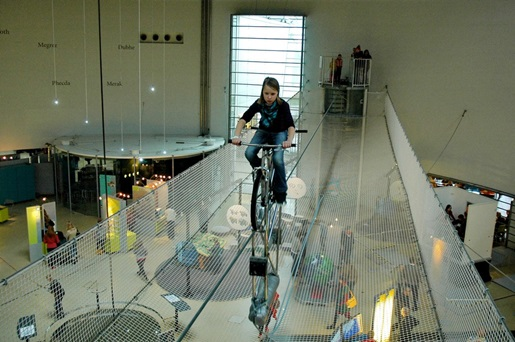
\includegraphics[width=0.75\linewidth]{chapters/chapter8/images/9}
		\caption{}
		\label{ris:image8x9}
	\end{center}
\end{figure}

Упражнение для любознательных: Какой элемент представленной конструкции делает поездку безопасной?

Резюмируя наши знания об устойчивости и сцеплении с дорогой, можно дать две простые рекомендации по сборке любых ваших роботов. Основная масса должна быть всегда сосредоточена над ведущими колесами и как можно ниже!